\section*{Introduction}
\addcontentsline{toc}{section}{Introduction}

This sprint delivers the administration layer, multi-language support, and
in-app onboarding tutorials that complete the \domainterm{MES} solution.
Administrators receives access to an activity log, and a user role management
interface. Quality-of-life features include full internationalisation with English,
French, and Arabic support, automatic right-to-left layout for Arabic, and guided 
coach-mark tutorials shown once in the main screens on first use. This sprint also 
delivers machine performance dashboard for the \userrole{Supervisor}. No new
\techname{Business Central} tables are introduced in this sprint; all data is
derived by querying and aggregating the tables created in Sprints~1 through~3.

% ---------------------------------------------------------------------------
% 1. SPRINT BACKLOG
% ---------------------------------------------------------------------------
\section{Sprint Backlog}

This sprint covers \textbf{Domain 4:}
\textbf{\domainterm{Administration \& Monitoring}}

% ----------------------------------------------------------
%  US-4.1
% ----------------------------------------------------------
\begin{longtable}{@{} P{0.09\linewidth} P{0.34\linewidth} P{0.53\linewidth} @{}}
      \caption{Sprint 4 Story Backlog}
      \label{tab:s4-sprint-backlog} \\
      \toprule
      \textbf{ID} & \textbf{User Story} & \textbf{Tasks} \\
      \midrule
      \endfirsthead
      \toprule
      \textbf{ID} & \textbf{User Story} & \textbf{Tasks} \\
      \midrule
      \endhead
      \multicolumn{3}{r}{\small Continued on next page} \\
      \endfoot
      \bottomrule
      \endlastfoot
            
      \textbf{US-4.1}
      & As an \userrole{Supervisor}, I need a performance dashboard for all
      machines so that I can monitor production health across the facility.
      & \noindent\textit{Business Central (AL):}
      \begin{itemize}[noitemsep, topsep=0pt, partopsep=0pt, leftmargin=*]
            \item Create function \texttt{fetchMachineDashboard()} in codeunit \techname{MES Machine Fetch}.
            \item Expose the function through the codeunit \techname{MES Web Service}.
      \end{itemize}
      \\ & &
      \noindent\textit{Flutter:}
      \begin{itemize}[noitemsep, topsep=0pt, partopsep=0pt, leftmargin=*]
            \item Create model \techname{MachineDashboardModel}.
            \item Create \techname{LogService} to consume the \texttt{fetchMachineDashboard} API and \techname{LogProvider} to manage its state.
            \item Create page \techname{MachineDashboardPage}.
            \item Implement machine dashboard search and time-range filtering in \techname{MachineDashboardPage}.
      \end{itemize} \\  
      \midrule 
      \textbf{US-4.2}
      & As an \userrole{Administrator}, I need a filterable log of all
      system actions so that I can audit operator and machine activity.
      & \noindent\textit{Business Central (AL):}
      \begin{itemize}[noitemsep, topsep=0pt, partopsep=0pt, leftmargin=*]
            \item Create function \texttt{fetchActivityLog()} in codeunit \techname{MES Machine Fetch}.
            \item Add the wrapper of the function to \techname{MES Web Service}.
      \end{itemize}
      \\ & &
      \noindent\textit{Flutter:}
      \begin{itemize}[noitemsep, topsep=0pt, partopsep=0pt, leftmargin=*]
            \item Create model \techname{ActivityLogModel}.
            \item Create \techname{LogService} to consume the \texttt{fetchActivityLog()} API and \techname{LogProvider} to manage its state.
            \item Create page \techname{ActivityLogPage}.
            \item Implement activity log search, type filtering, time-range filtering, and pagination in \techname{ActivityLogPage}.
      \end{itemize} \\
      \midrule
      \textbf{US-4.3}
      & As any user, I need the application available in English, French, and
      Arabic so that I can use it in my preferred language.
      & \noindent\textit{Flutter:}
      \begin{itemize}[noitemsep, topsep=0pt, partopsep=0pt, leftmargin=*]
            \item Integrate the \texttt{easy\_localization} package.
            \item Create translation JSON files for \texttt{en}, \texttt{fr}, and \texttt{ar}.
            \item Create widget \techname{LanguageSelector}.
            \item Implement language selection in \techname{ProfilePage}.
            \item Add the \techname{EasyLocalization} wrapper in \texttt{main()}.
            \item Implement right-to-left layout support through \texttt{MaterialApp}.
      \end{itemize} \\
      \midrule
      \textbf{US-4.4}
      & As a first-time user, I need guided coach-mark tutorials so that I can
      learn the interface without external documentation.
      & \noindent\textit{Flutter:}
      \begin{itemize}[noitemsep, topsep=0pt, partopsep=0pt, leftmargin=*]
            \item Integrate the \texttt{tutorial\_coach\_mark} package.
            \item Implement tutorial persistence using \techname{SharedPreferences}.
            \item Create \techname{MachineListTutorial}, \techname{MachineDetailTabsTutorial}, \techname{OperationDetailTutorial}, and \techname{AdminDashboardTutorial}.
            \item Implement tutorial target styling and localisation.
      \end{itemize} \\
\end{longtable}
% ---------------------------------------------------------------------------
% 2. BUSINESS RULES
% ---------------------------------------------------------------------------
\section{Design}

\subsection{Use Case Diagram}

The UML Use Case Diagram (Figure~\ref{fig:s4-use-case-s4}) covers the actors and
interactions introduced in this sprint. The \userrole{Administrator} gains the
interaction \uilabel{View Activity Log}.The \userrole{Supervisor} gains the interaction
\uilabel{View Machine Dashboard}. All three actors (\userrole{Operator},
\userrole{Supervisor}, \userrole{Administrator}) share the
\uilabel{Select Language} and \uilabel{View Tutorial} use cases, which are
cross-cutting accessibility features available on every screen.

\begin{figure}[H]
      \centering
      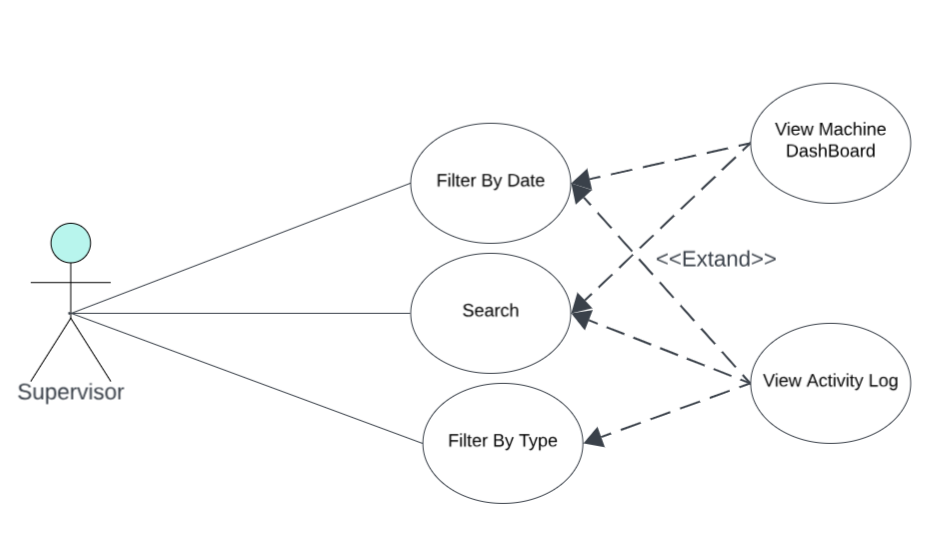
\includegraphics[height=0.5\textheight,keepaspectratio]{./media/MES_Sprint-4-Report/diagrams/useCase/sprint4.png}
      \caption{UML Use Case Diagram --- Administration \& UX.}
      \label{fig:s4-use-case-s4}
\end{figure}

\subsection{Textual Use Case Description}

The following table (Table~\ref{tab:s4-uc-scan-component-s4}) provides the detailed
textual description of the \textit{View Machine Dashboard} use case, which
represents the most significant new administrator workflow in this sprint.

\Needspace{8\baselineskip}
\begin{longtable}{@{} P{0.21\linewidth} P{0.75\linewidth} @{}}
            
      \caption{Textual Use Case Description --- View Machine Dashboard}
      \label{tab:s4-uc-scan-component-s4} \\
      \toprule
      \endfirsthead
      \midrule
      \endhead
      \multicolumn{2}{r}{\small Continued on next page} \\
      \endfoot
      \bottomrule
      \endlastfoot
      
      \textbf{Use Case Name}  & View Machine Dashboard   \\
      \midrule
      \textbf{Primary Actor}  & \userrole{Supervisor} \\
      \midrule
      \textbf{Preconditions}  &                          
      \begin{itemize}[noitemsep, topsep=0pt, partopsep=0pt, leftmargin=*]
      \item The user is authenticated with the \domainterm{Supervisor} role.
      \end{itemize} \\
      \midrule
      \textbf{Postconditions} &                          
      \begin{itemize}[noitemsep, topsep=0pt, partopsep=0pt, leftmargin=*]
      \item A grid of machine cards is displayed, each showing uptime, production
      totals, and scrap for the selected time window.
      \item Changing the time-range selector refreshes all card metrics.
      \end{itemize} \\
      \midrule
      \textbf{Main Scenario}  &                          
      \begin{enumerate}[noitemsep, topsep=0pt, partopsep=0pt, leftmargin=*]
      \item The Supervisor logs in and is routed to \techname{machineList}.
      \item The Supervisor selects \uilabel{Machine Dashboard} in the topBar.
      \item The system POSTs to \apiendpoint{/MESWebService\_fetchMachineDashboard}
      with the default \texttt{hoursBack = 24}.
      \item The backend aggregates execution and progression records and returns
      per-machine metrics.
      \item The Supervisor changes the time range to 48\,h via the AppBar
      dropdown; the page re-fetches and updates.
      \end{enumerate} \\
            
\end{longtable}

\subsection{Sequence Diagrams}

The following sequence diagrams illustrate the communication flow between the
\techname{Flutter} frontend, the \techname{Business Central} OData layer, and
the \techname{AL} business logic for the administrator analytics flows
introduced in Sprint~4.

Figure~\ref{fig:s4-seq-fetch-dashboard} depicts the machine dashboard retrieval
flow. The \techname{AL} layer iterates over all \domainterm{Machine Center}
records and, for each machine, computes the total operation count, cancelled/Interrupted operations,
total production and scrap quantities, and uptime percentage from the corresponding
\techname{Business Central} records before assembling the per-machine KPI rows
returned to the \techname{Flutter} client.

\begin{figure}[H]
      \centering
      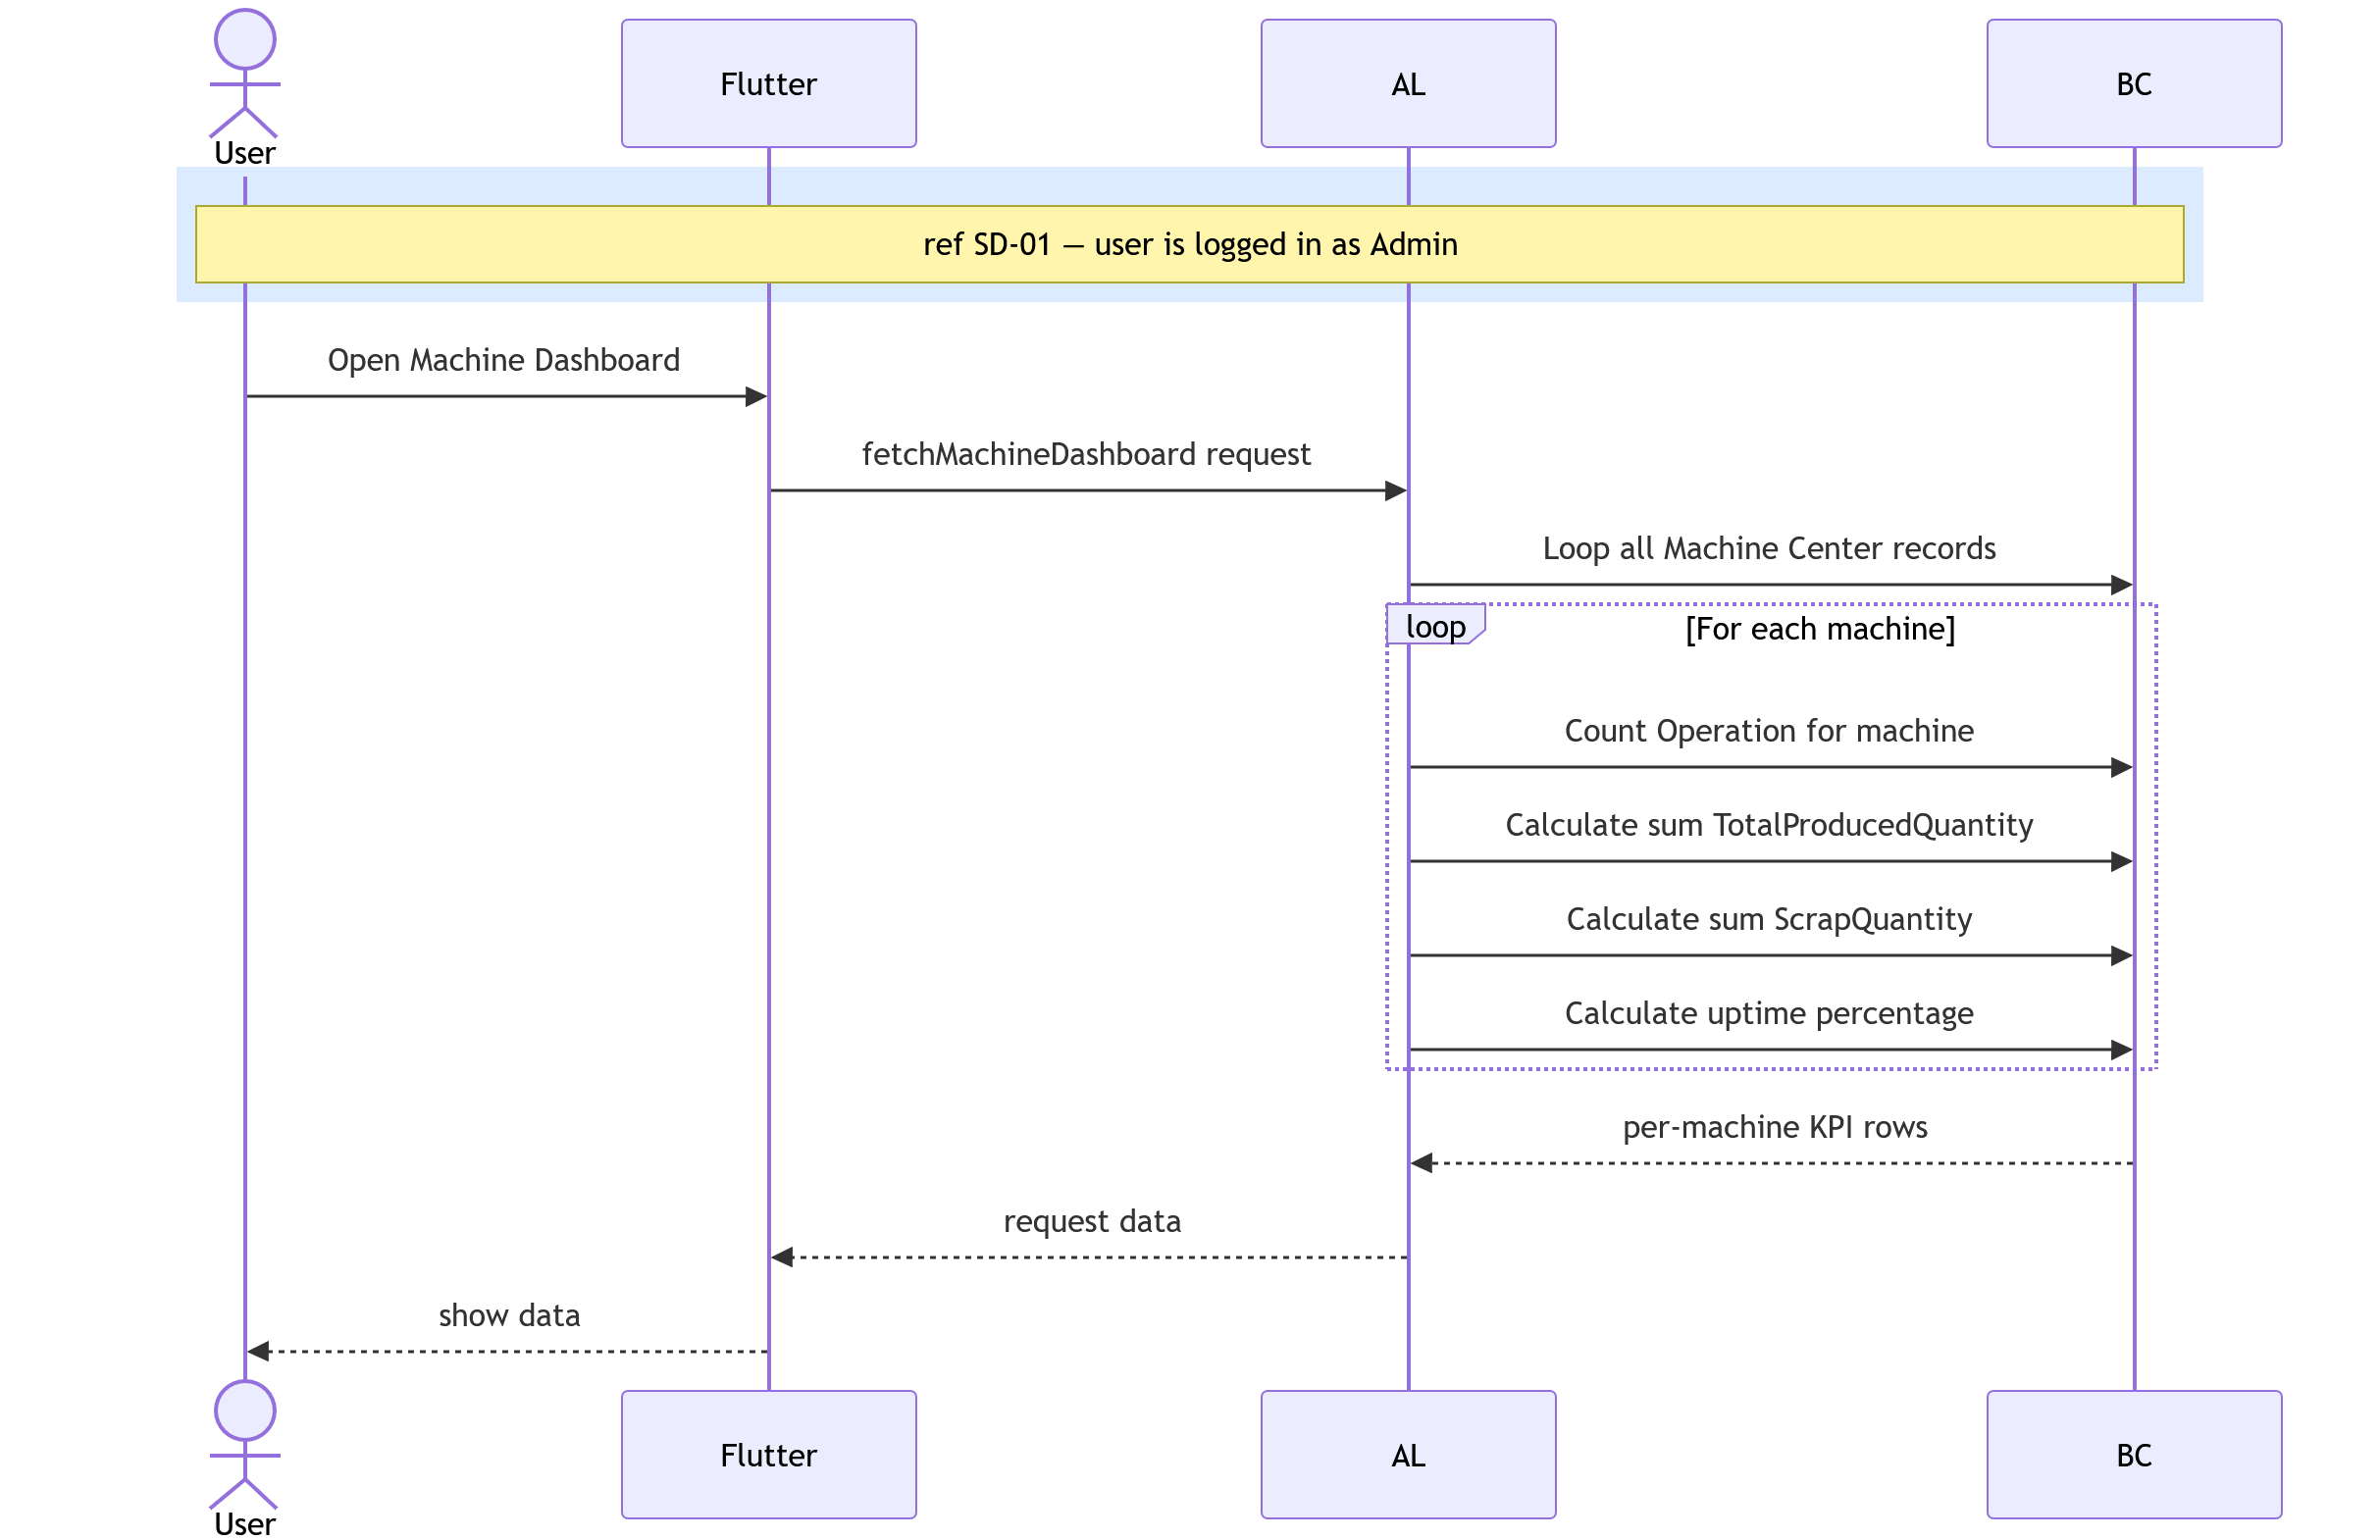
\includegraphics[width=\linewidth,height=0.82\textheight,keepaspectratio]{./media/MES_Sprint-4-Report/diagrams/sequence/machine-dashboard.png}
      \caption{SD-19: Fetch Machine Dashboard.}
      \label{fig:s4-seq-fetch-dashboard}
\end{figure}

%=====SD-19==========================================================
% sequenceDiagram
%       actor User
%       participant Flutter
%       participant Node as Node.js Middleware
%       participant AL
%       participant BC

%       rect rgb(220,235,255)
%           Note over User,BC: ref SD-01 — user is logged in as Admin
%       end

%       User->>Flutter: Open Machine Dashboard
%       Flutter->>Node: POST /api/fetchMachineDashboard 
%       Node->>AL: MESWebService_fetchMachineDashboard 

%       AL->>BC: filter machines to relevant WCs only
%       BC-->>AL: filtered machine list

%       loop For each machine in filtered list
%           AL->>BC: collect the detail from all the necessary records 
%           BC-->>AL: per-machine aggregated KPIs
%       end

%       AL-->>Node: response
%       Node-->>Flutter: response
%       Flutter-->>User: Machine dashboard grid rendered
%====================================================================

Figure~\ref{fig:s4-seq-fetch-activity-log} presents the activity log retrieval
flow. The \techname{AL} layer queries four event tables in parallel;
\domainterm{MES Operation State}, \domainterm{MES Operation Progression},
\domainterm{MES Operation Scrap}, and \domainterm{MES Component Consumption}
, filtering each by the requested time window. For every event row it joins
the associated \domainterm{MES User} and \domainterm{MES Operation Execution}
records to enrich the entry with operator identity and execution context. The
resulting flat event list is returned to the \techname{Flutter} client, which
renders it as a chronological activity table.


\begin{figure}[H]
      \centering
      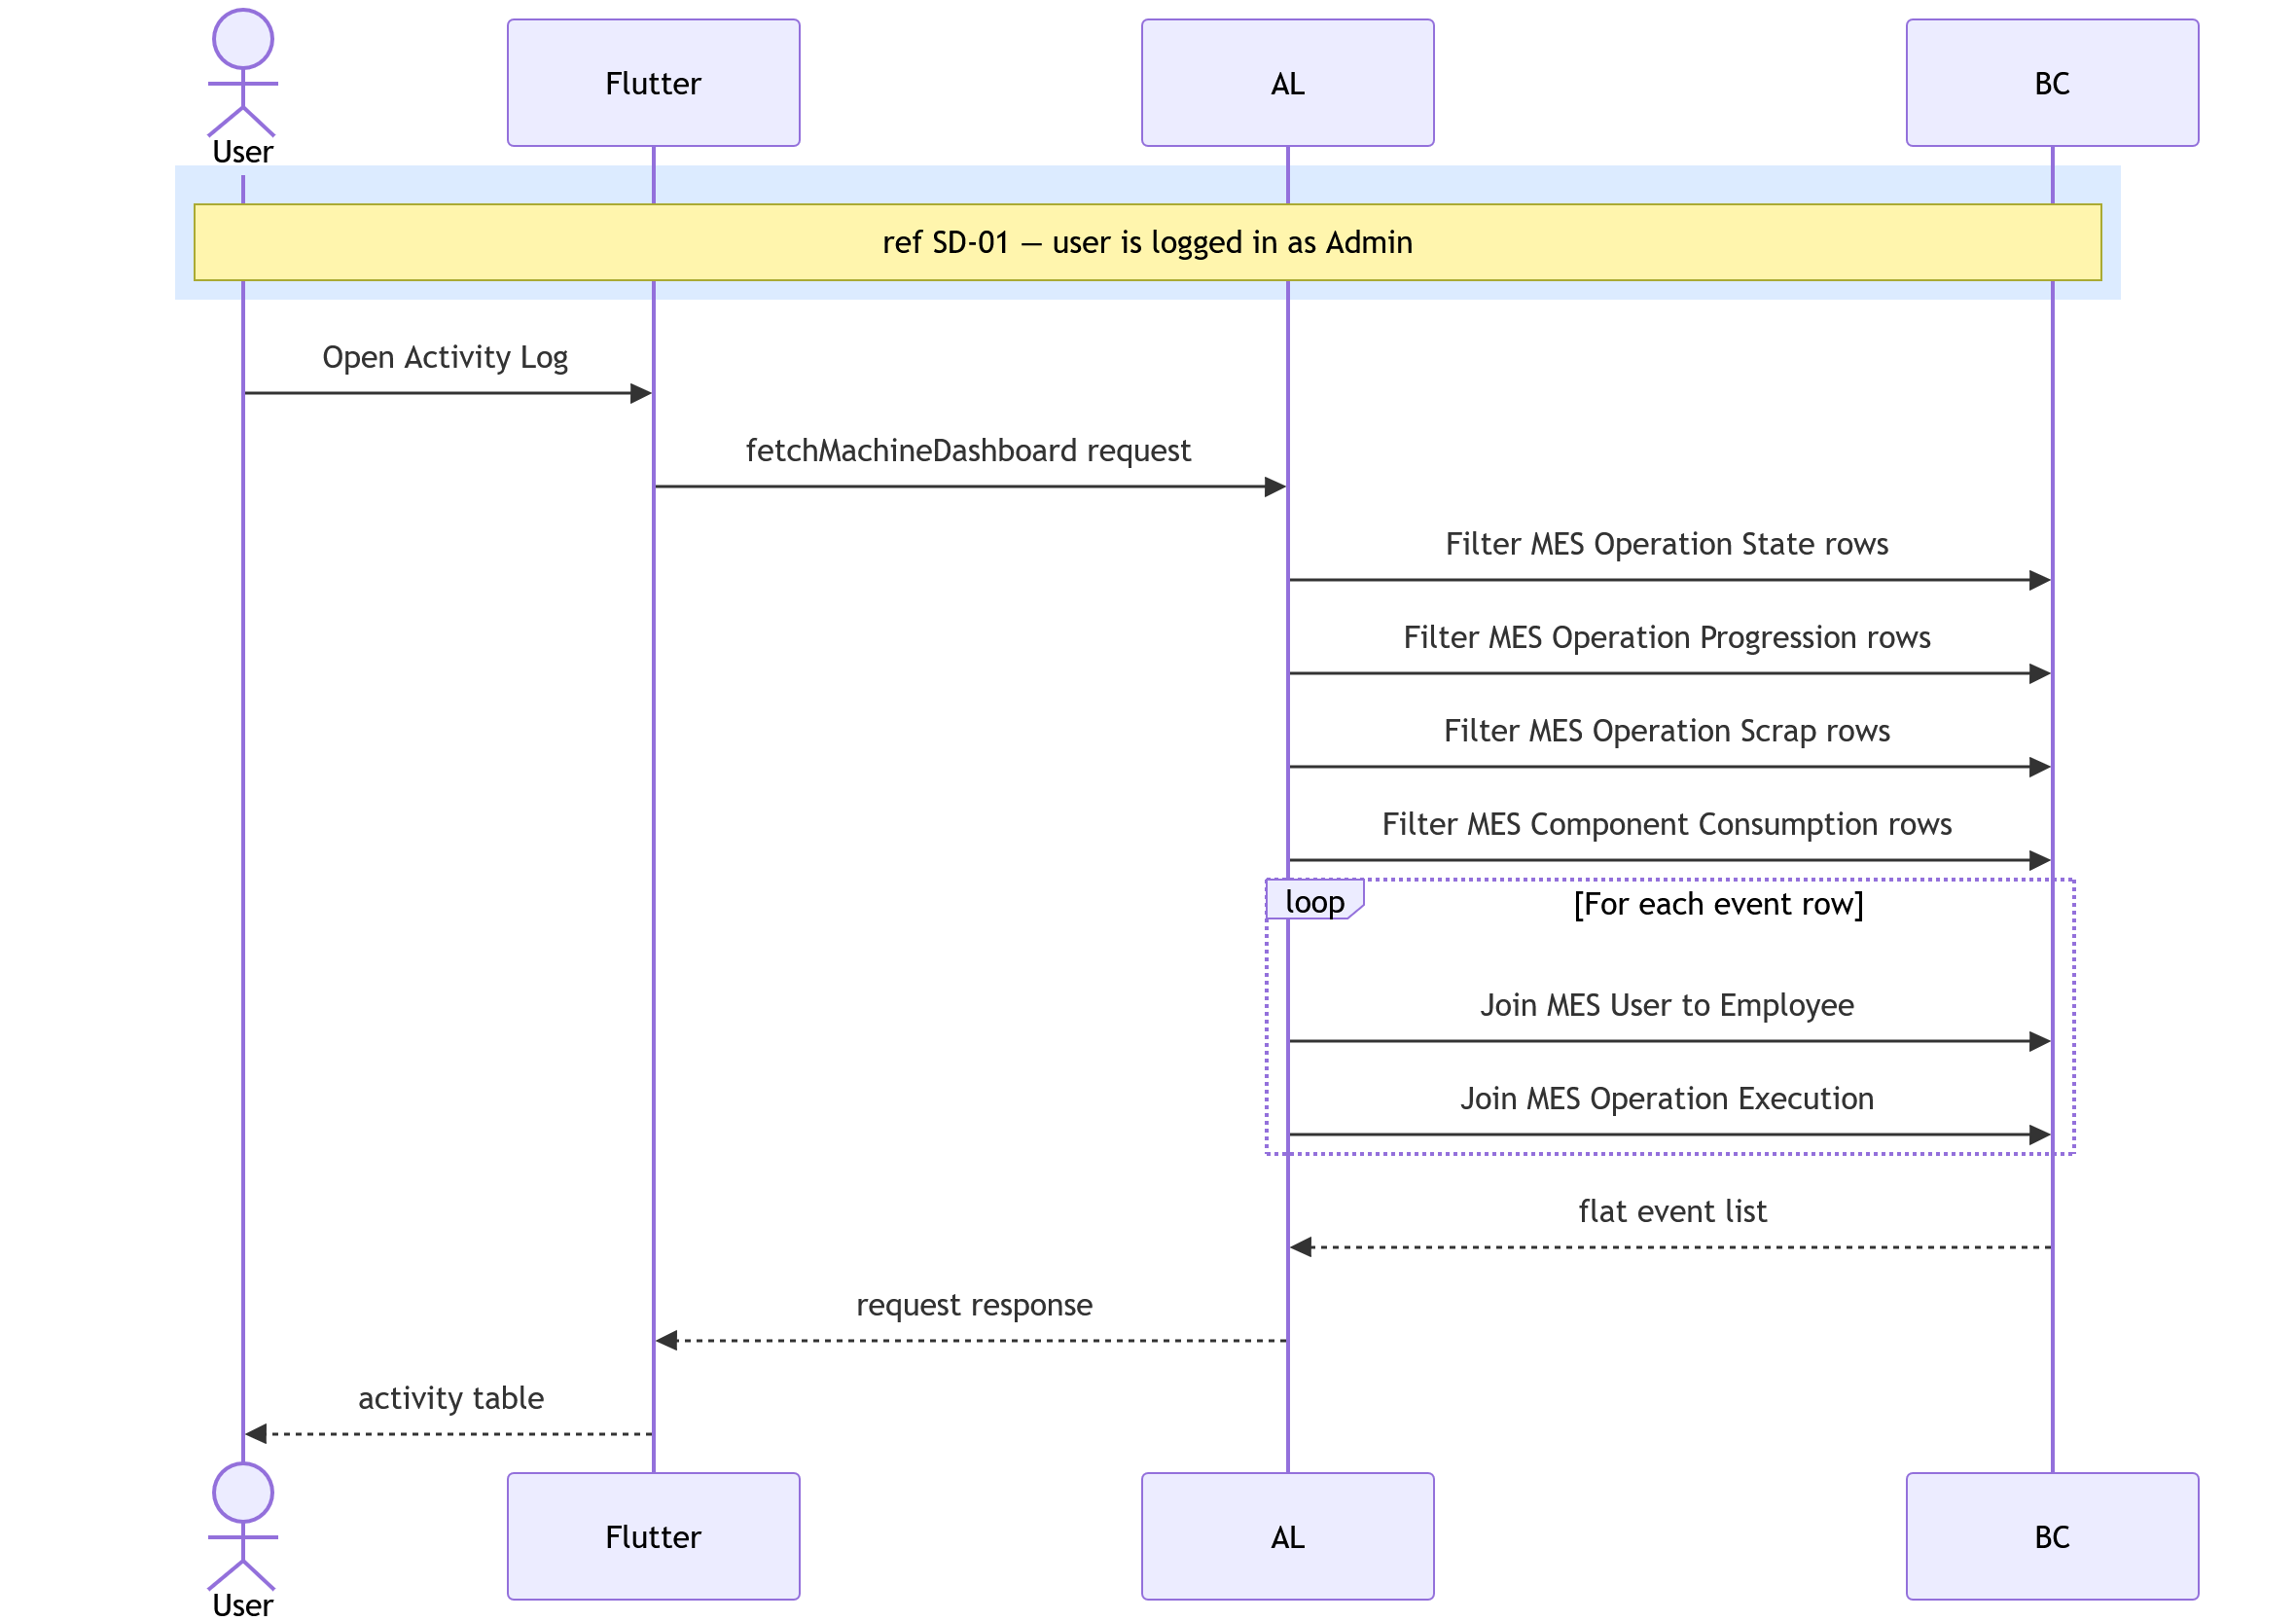
\includegraphics[width=\linewidth,height=0.82\textheight,keepaspectratio]{./media/MES_Sprint-4-Report/diagrams/sequence/activity-log.png}
      \caption{SD-20: Fetch Activity Log.}
      \label{fig:s4-seq-fetch-activity-log}
\end{figure}

%=====SD-20==========================================================
% sequenceDiagram
%       actor User
%       participant Flutter
%       participant Node as Node.js Middleware
%       participant AL
%       participant BC

%       rect rgb(220,235,255)
%           Note over User,BC: ref SD-01 — user is logged in as Admin
%       end

%       User->>Flutter: Open Activity Log 
%       Flutter->>Node: POST /api/fetchActivityLog 
%       Node->>AL: MESWebService_fetchActivityLog 

%       AL->>BC: collect Operation state changes within the cutoff
%       AL->>BC: collect the Operation progress within the cutoff
%       AL->>BC: collect the scrap declarations within the cutoff
%       AL->>BC: collect the component scan within the cutoff

%       AL->>BC: resolve the name of the users


%       AL->>AL: Merge all four event lists into flat chronological array
%       AL-->>Node: response
%       Node-->>Flutter: response
%       Flutter-->>User: Activity log table rendered
%====================================================================

\subsection{Class Diagram}

\begin{figure}[H]
	\centering
	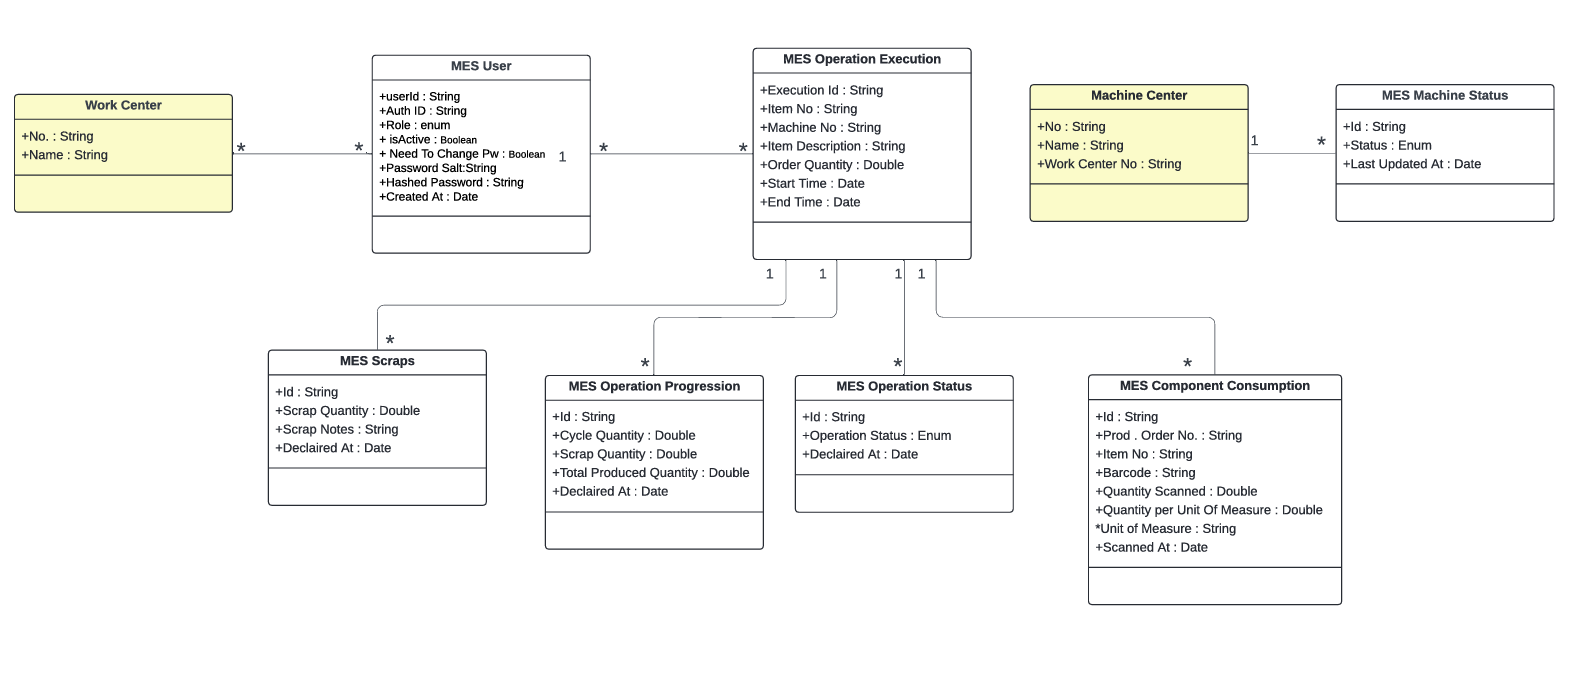
\includegraphics[width=\linewidth,keepaspectratio]{./media/MES_Sprint-4-Report/diagrams/class/sprint4.png}
	\caption{UML Class Diagram.}
	\label{fig:s4-class-diagram}
\end{figure}

% ---------------------------------------------------------------------------
% 4. IMPLEMENTATION
% ---------------------------------------------------------------------------
\section{Implementation}

\subsection{Backend Implementation}

No new \techname{Business Central} tables are introduced in this sprint.
All backend work consists of new query and aggregation procedures added to
\techname{MES Web Service} (codeunit~50126), reading from tables defined in
Sprints~1 through~3.

\subsubsection{Dashboard Aggregation}

\texttt{fetchMachineDashboard()} accepts a \texttt{hoursBack} window and an
optional \texttt{workCenterNoJson} filter. For each \modulename{Machine Center}
it aggregates the matched \modulename{MES Operation Execution} records,
summing \texttt{Cycle Quantity} from linked \modulename{MES Operation
Progression} entries to obtain total produced and scrap counts, and computing
uptime as \texttt{runningMinutes / (hoursBack × 60) × 100}, capped at 100.

\subsubsection{Activity Log Aggregation}

\texttt{fetchActivityLog()} queries four tables within the \texttt{hoursBack}
window --- \modulename{MES Operation State}, \modulename{MES Operation
Progression}, \modulename{MES Operation Scrap}, and \modulename{MES Component
Consumption} --- resolves operator names via the \modulename{Employee} table,
and merges the results into a single descending-timestamp JSON array.

\subsubsection{API Endpoints Added in Sprint 4}

All endpoints are exposed as ODataV4 unbound actions through
\techname{MES Web Service} (codeunit~50126) and are served by the
middleware at:

\begin{center}
  \texttt{middlewareHostURL/api/<endpointName>}
\end{center}

\noindent Each request is forwarded to the \techname{AL} layer as an
ODataV4 action call of the form:

\begin{center}
  \texttt{POST~<baseUrl>/ODataV4/MESWebService\_<ProcedureName>?company=<companyId>}
\end{center}

\begin{longtable}{@{} P{0.48\linewidth} @{\hspace{0.04\linewidth}} P{0.48\linewidth} @{}}
  \caption{New API Endpoints --- Sprint 4}
  \label{tab:s4-api-endpoints}\\
  \toprule
  \textbf{Endpoint} & \textbf{Endpoint}\\
  \midrule
  \endfirsthead
  \toprule
  \textbf{Endpoint} & \textbf{Endpoint}\\
  \midrule
  \endhead
  \multicolumn{2}{r}{\small Continued on next page}\\
  \endfoot
  \bottomrule
  \endlastfoot

  \apiendpoint{fetchMachineDashboard} & \apiendpoint{fetchActivityLog} \\ 
\end{longtable}

\subsection{Frontend Implementation}

\subsubsection{Shared HTTP Infrastructure}

All sprint services (including retroactively migrated ones) share a
\techname{HttpClient} and \techname{HttpResponseParser} layer, replacing
the inline \texttt{http.post} calls from Sprint~1.
\techname{HttpClient.post()} is a centralised wrapper that injects
JSON headers and encodes the request body.
\techname{HttpResponseParser} exposes four static helpers:
\texttt{parseList()} and \texttt{parseObject()} decode OData list and
single-object responses respectively; \texttt{parseWriteResult()} decodes
write responses and surfaces backend errors; \texttt{\_assertSuccess()}
validates HTTP status codes and throws a structured exception on non-2xx
responses.

\subsubsection{Provider Architecture}

\begin{longtable}{@{} P{0.30\linewidth} P{0.65\linewidth} @{}}
  \caption{Provider Responsibilities --- Sprint 4 Additions}
  \label{tab:s4-providers-s4} \\
  \toprule
  \textbf{Provider}             & \textbf{Responsibility} \\
  \midrule
  \endfirsthead
  \toprule
  \textbf{Provider}             & \textbf{Responsibility} \\
  \midrule
  \endhead
  \multicolumn{2}{r}{\small Continued on next page} \\
  \endfoot
  \bottomrule
  \endlastfoot

  \techname{LogProvider}        &
   Owns dashboard and activity log fetch calls; exposes \texttt{selectedHours},
   \texttt{hourOptions}, and \texttt{setHours()} shared between the two admin pages. \\
  \addlinespace
  \techname{MesBarcodeProvider} & 
  Exposes \texttt{fetchAllBarcodes()}; resolves the session token automatically from
  \techname{AuthProvider}. \\
\end{longtable}

\subsubsection{User Interface}


\begin{figure}[H]
  \centering
  \setlength{\fboxsep}{5pt}
  \colorbox{black}{%
    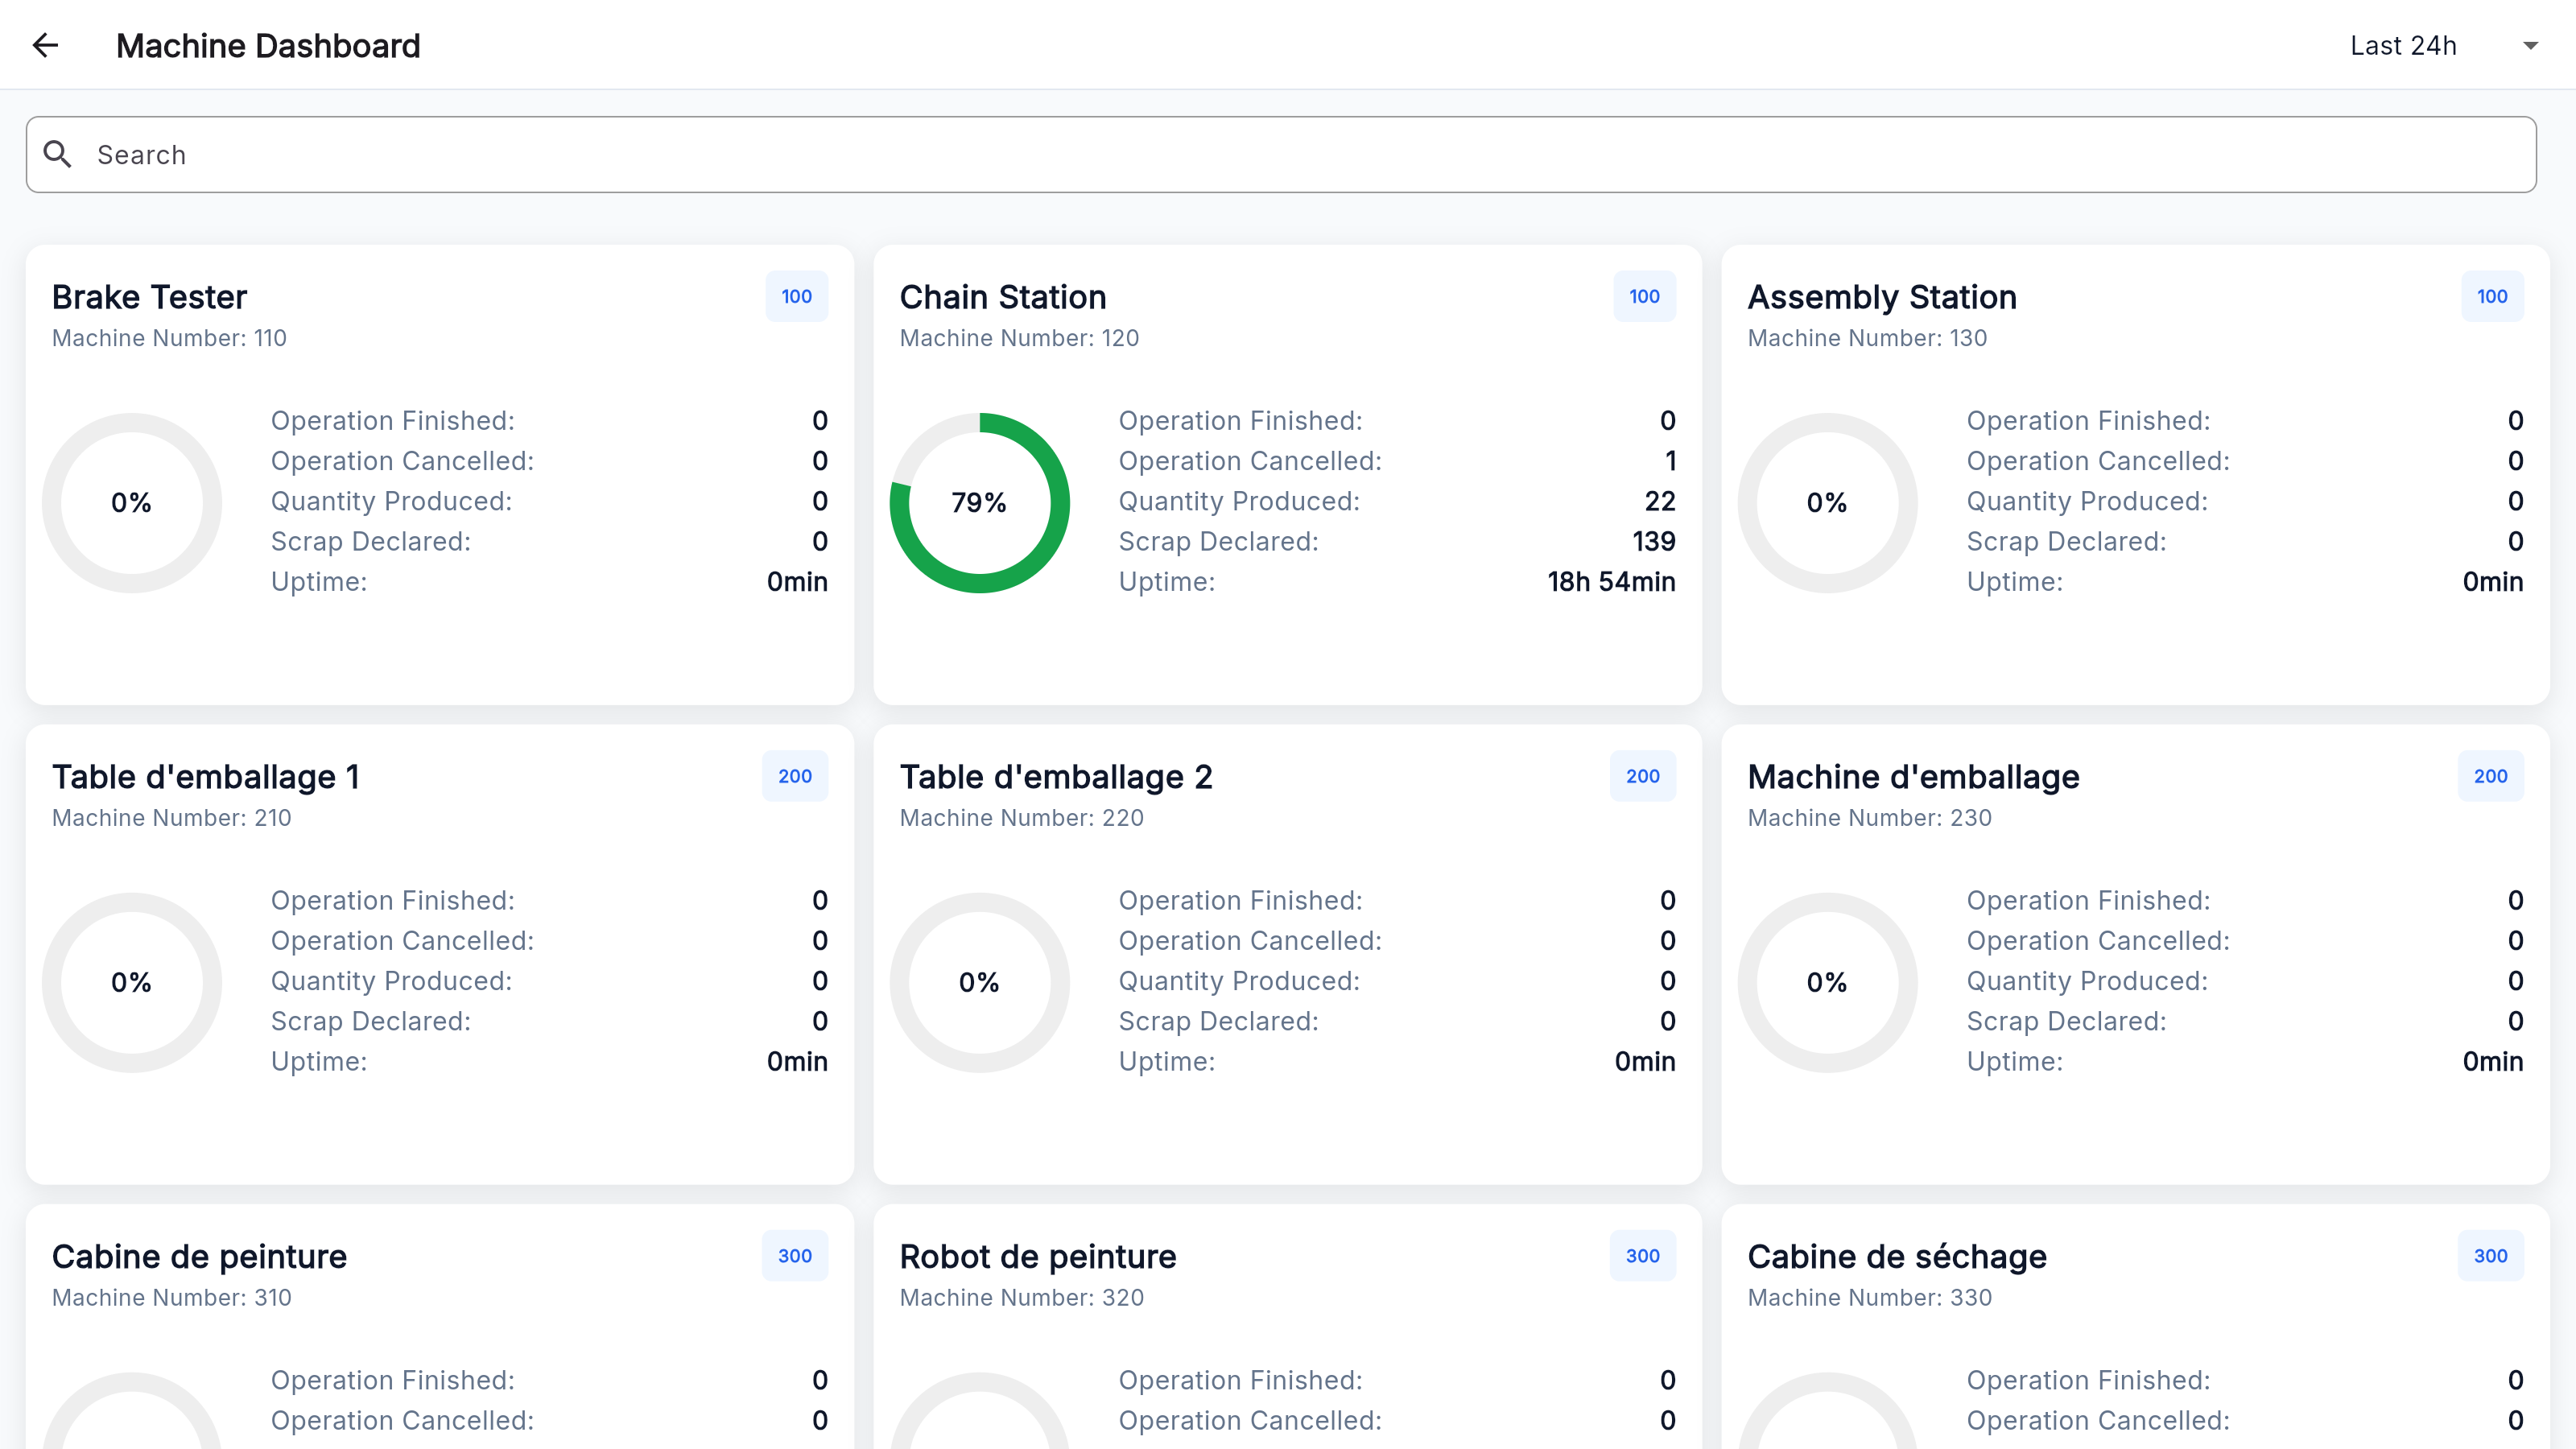
\includegraphics[height=0.3\textheight,keepaspectratio]{./media/MES_Sprint-4-Report/UI/dashboard/wide.png}%
    \hspace{\fboxsep}%
    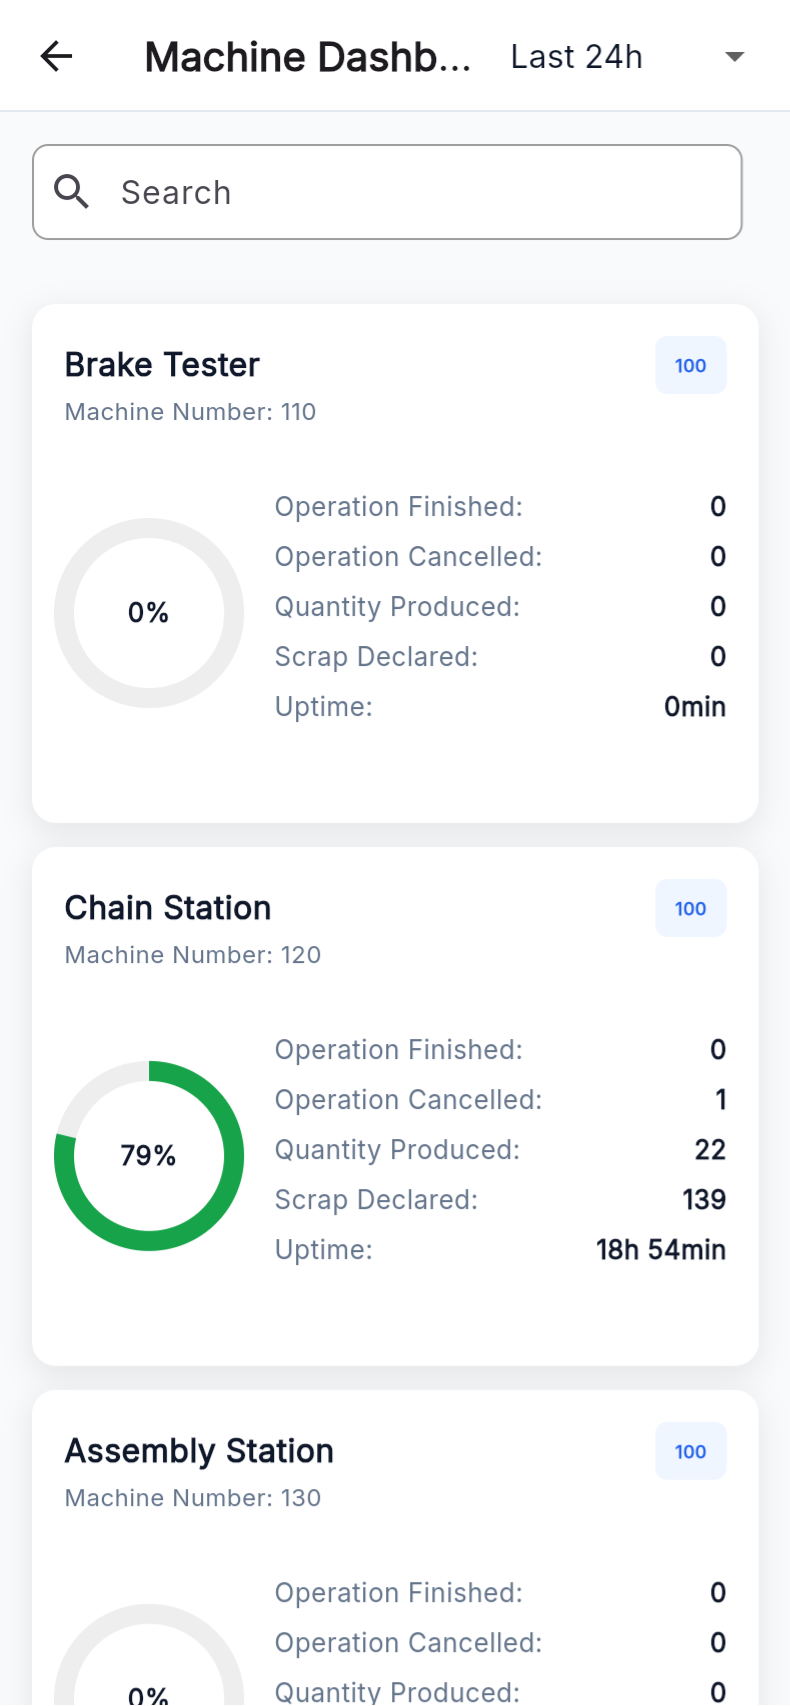
\includegraphics[height=0.3\textheight,keepaspectratio]{./media/MES_Sprint-4-Report/UI/dashboard/small.png}%
  }
  \caption{\uilabel{Machine Dashboard Page} --- desktop and mobile views.}
  \label{fig:s4-ui-machine-dashboard}
\end{figure}

Figures~\ref{fig:s4-ui-machine-dashboard} and~\ref{fig:s4-ui-activity-log} illustrate
the two pages. The \uilabel{Machine Dashboard Page} renders one card per machine
with a circular uptime indicator and four metric rows (finished operations, 
Cancelled and Interrupted operations, produced, scrap, uptime), and
an AppBar time-range dropdown that re-fetches on change. The \uilabel{Activity Log Page}
presents a paginated, newest-first event list where each row shows a type icon, 
operator, machine, and expandable action text; AppBar dropdowns filter by type and 
time range.

\begin{figure}[H]
  \centering
  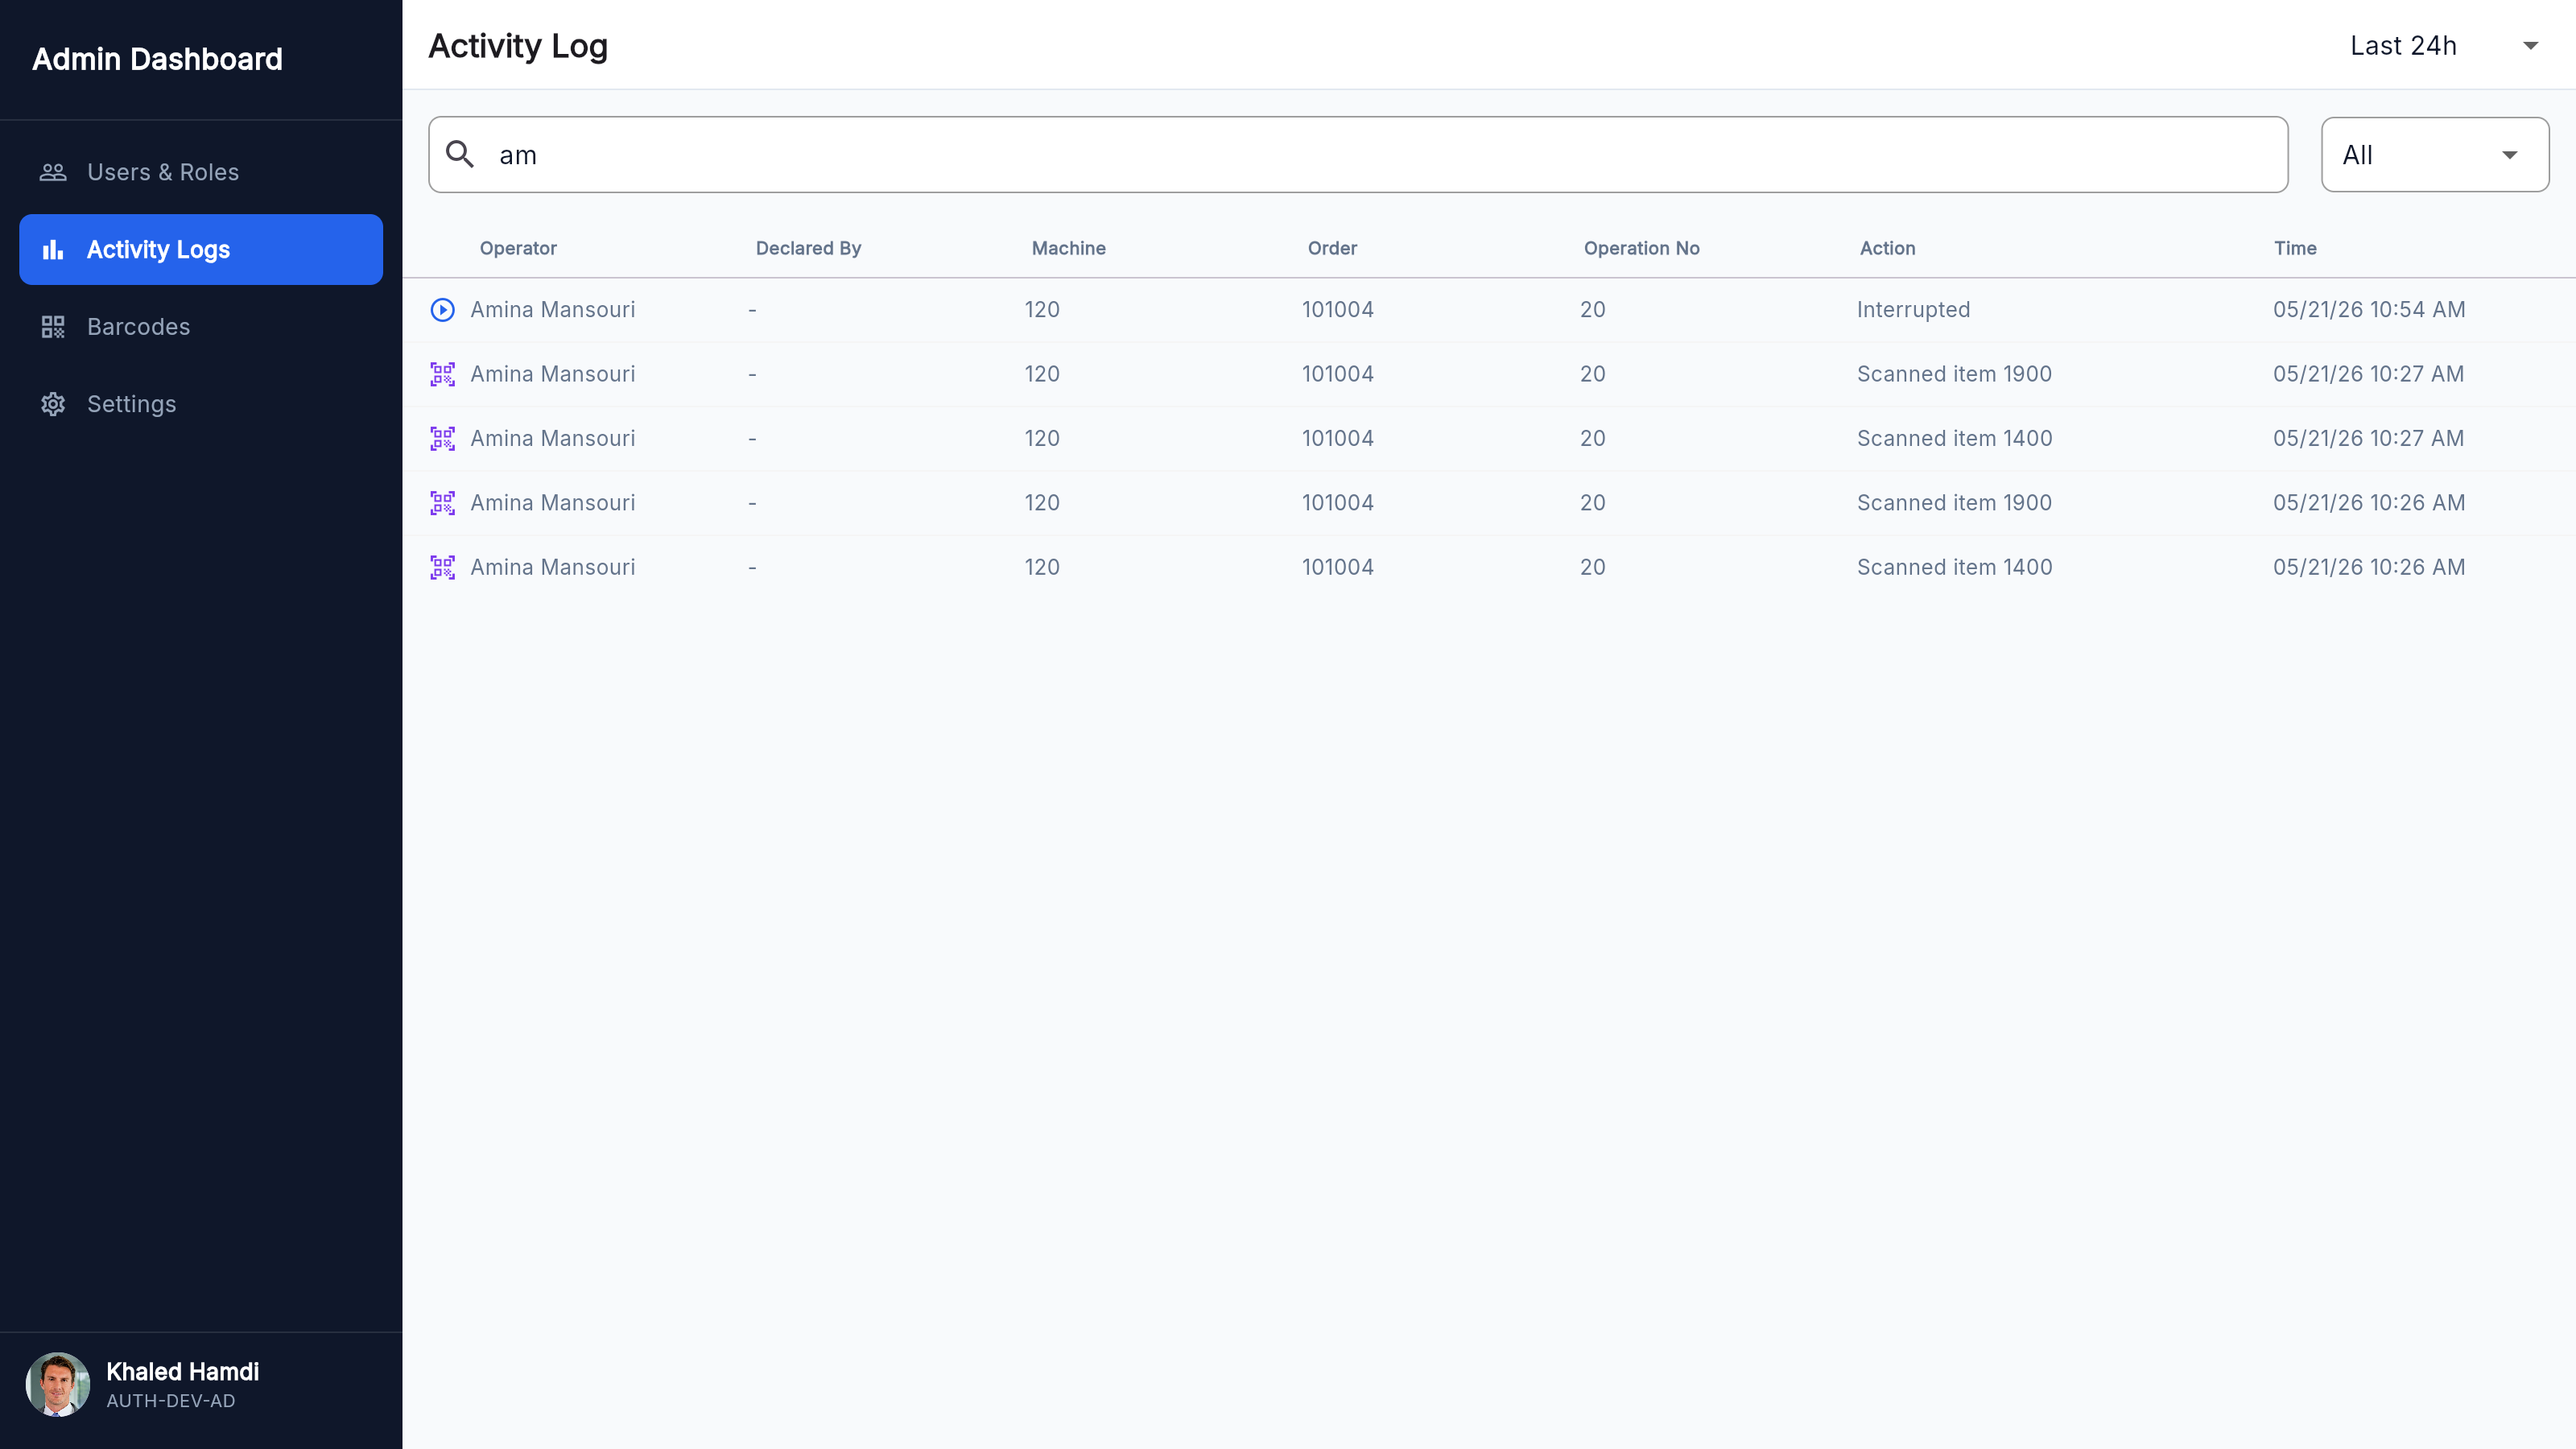
\includegraphics[height=0.3\textheight,keepaspectratio]{./media/MES_Sprint-4-Report/UI/activityLog/wide.png}
  \caption{\uilabel{Activity Log Page} --- desktop and mobile views.}
  \label{fig:s4-ui-activity-log}
\end{figure}
\section{Test and validation}
\subsection{Integration test}

For integration testing, we chose Postman, a powerful and user-friendly tool for API evaluation. Figure~\ref{fig:s4-test-postman-activityLog} shows a test case for the \apiendpoint{/activityLog} endpoint.

\begin{figure}[H]
  \centering
  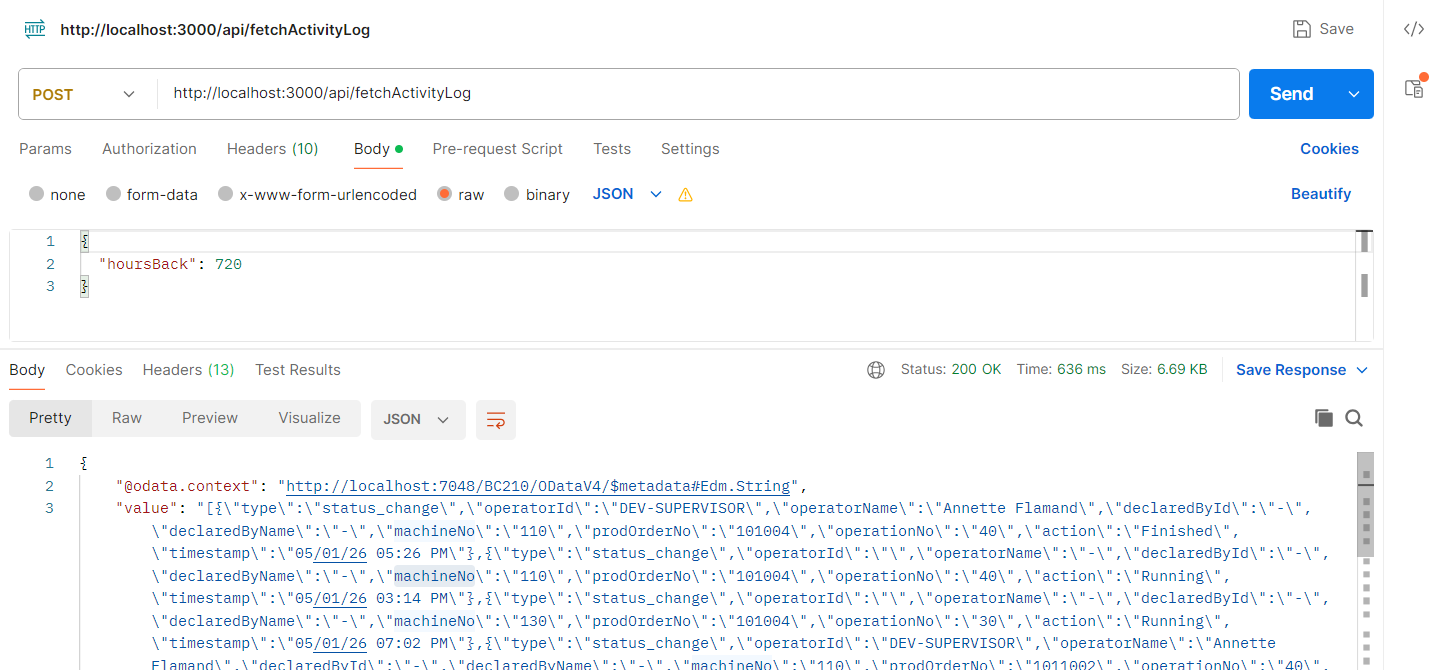
\includegraphics[width=\linewidth,keepaspectratio]{./media/MES_Sprint-4-Report/test/postman/fetchActivityLog.png}
  \caption{Postman endpoint test --- fetchActivityLog.}
  \label{fig:s4-test-postman-activityLog}
\end{figure}

Figure~\ref{fig:s4-test-postman-machineDashboard} shows a test case for the \apiendpoint{/MachineDashboard} endpoint.

\begin{figure}[H]
  \centering
  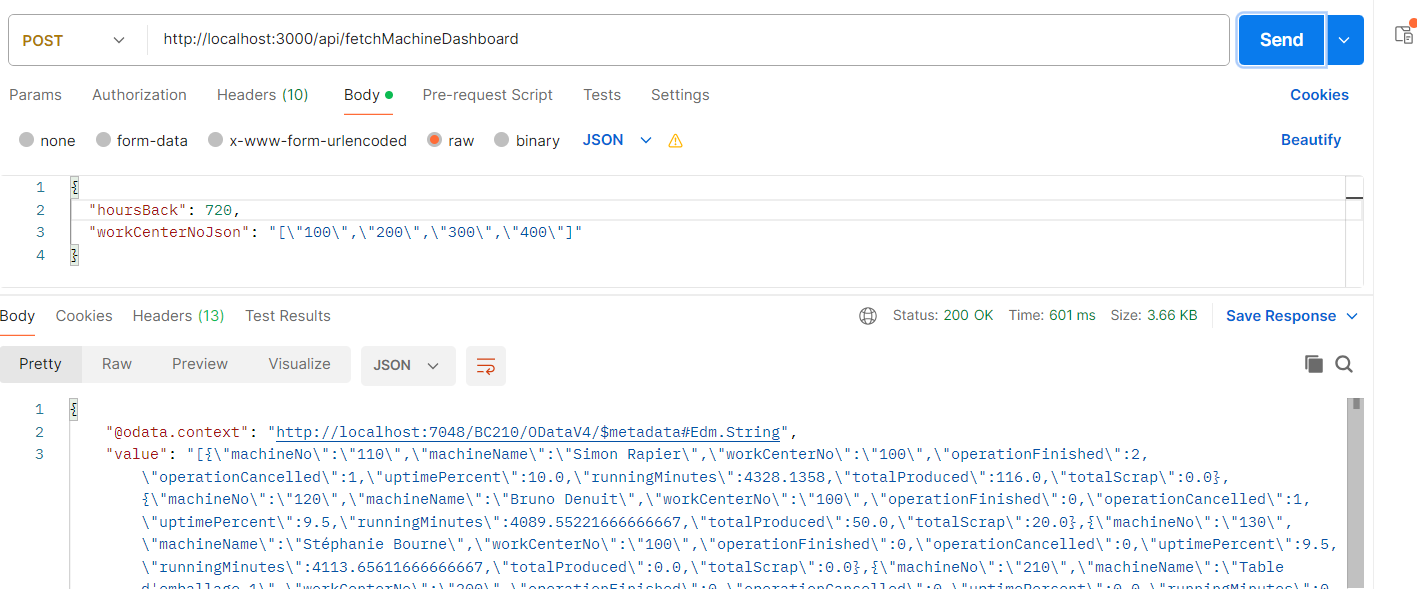
\includegraphics[width=\linewidth,keepaspectratio]{./media/MES_Sprint-4-Report/test/postman/fetchMachineDashboard.png}
  \caption{Postman endpoint test --- fetchMachineDashboard.}
  \label{fig:s4-test-postman-machineDashboard}
\end{figure}

% ---------------------------------------------------------------------------
% CONCLUSION
% ---------------------------------------------------------------------------
\phantomsection
\section*{Conclusion}
\addcontentsline{toc}{section}{Conclusion}

This sprint completed the \domainterm{MES} solution by delivering the
administration layer and cross-cutting quality-of-life features. Administrators
can now monitor the production health of the entire facility through a
configurable machine performance dashboard, audit all operator and machine
actions through a paginated activity log, and manage users from a persistent
navigation shell without losing context between sections. All users benefit from
full internationalisation covering English, French, and Arabic with automatic
right-to-left layout, and from guided coach-mark tutorials that ease onboarding
for first-time users.
